% Preamble
%\documentclass[aspectratio=43,t,xcolor={usenames,dvipsnames}]{beamer}
\documentclass[aspectratio=43,t,xcolor={usenames,dvipsnames},handout]{beamer}

% Packages
\usepackage{beamerstyle}
\usepackage[utf8]{inputenc}

\usepackage[ruled,vlined,linesnumbered]{algorithm2e}
\usepackage{amsmath,amssymb}
\usepackage{todonotes}
\usepackage{mdframed}
\usepackage{csquotes}
\usepackage{listings}
\usepackage{hyperref}



\lstset{frame=lines,framesep=3pt,numbers=left,numberblanklines=false,basicstyle=\ttfamily\small}
\definecolor{blue}{RGB}{0, 74, 153}

\setbeamercolor{emph}{fg=blue}
\renewcommand<>{\emph}[1]{%
  {\usebeamercolor[fg]{emph}\only#2{\bfseries}#1}%
}



% Document
\title{gym-traffic}
\subtitle{Controlling traffic lights with Reinforcement Learning}
\author{Dominik Woiwode}
\date{24.03.2021}

\hypersetup{
    pdftitle={Controlling traffic lights with RL},
	pdfauthor={Dominik Woiwode},
	pdfsubject={Reinforcement Learning},
	pdfdisplaydoctitle=true,
}

\begin{document}
    \begin{frame}[c,noframenumbering]
        \titlepage
    \end{frame}
%    \maketitle
%    \setcounter{\framenumber}{1}
    \begin{frame}[c]{The Environment}
        \begin{columns}

            \column{0.35\textwidth}

        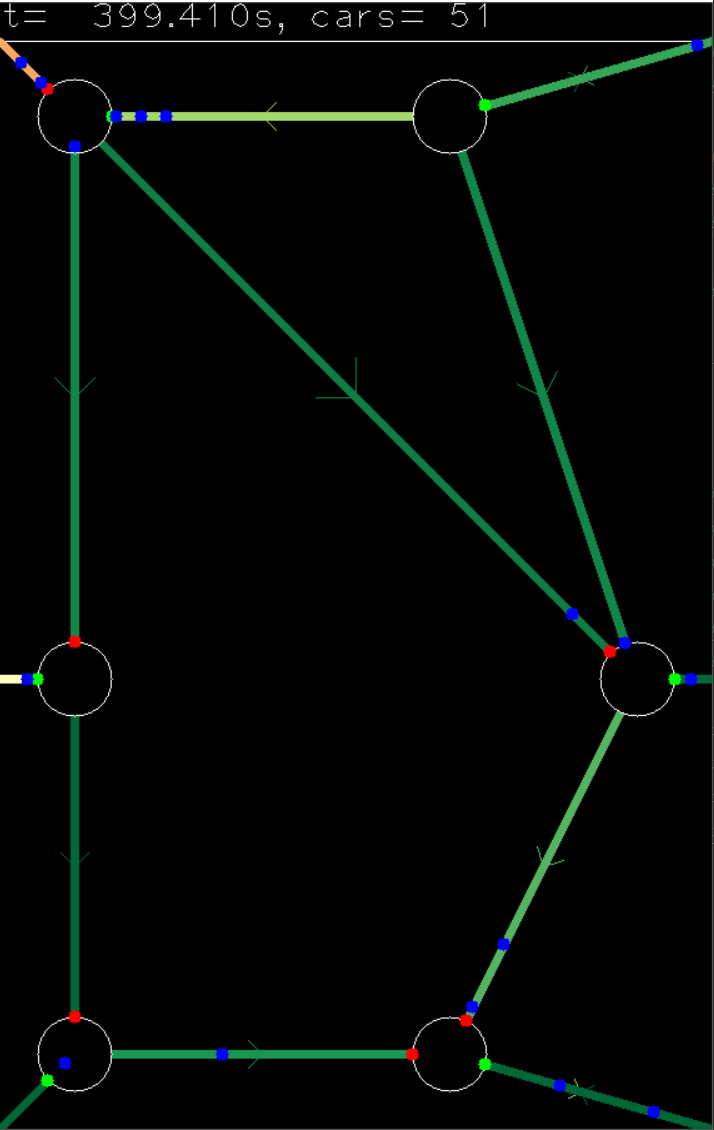
\includegraphics[width=1\textwidth]{images/environment}
%            \missingfigure[width=1.0\textwidth]{Image of environment}

            \column{0.65\textwidth}

            \begin{itemize}
                \item Street network as \emph{directed graph}
                \begin{itemize}
                    \item The world consists of multiple \emph{intersections}.
                    \item Intersections are connected with \emph{streets}.
                    \item Intersections have \emph{traffic lights} for each incoming street.
                    \item Traffic lights can either be \emph{red or green}.
                    \item For each intersection there \emph{cannot be more than one green light}.
                    \item \emph{Vehicles} can spawn at some intersections with a predefined route.
                    \item Vehicles drive on streets and \emph{stop at red traffic lights}.
                    \item Vehicles \emph{do not crash} into each other.
                \end{itemize}
                \item[$\leadsto$] \emph{An Agent has to control the traffic lights}.
                \begin{itemize}
                    \item \enquote{Traffic flow} should be maximized
                \end{itemize}
            \end{itemize}


        \end{columns}
    \end{frame}

    %%%%%%%%%%%%%%%%%%%%%%%%%%%%%%%%%%%%%%%%%%%%%%%%%%%%

    \begin{frame}[c]{Observation- and Actionspace}
        \begin{columns}
            \column{0.5\textwidth}
            \visible<1->{
            \textbf{Observationspace}
            \begin{itemize}
                \item For each intersection $t$:
                \begin{itemize}
                    \item For each incoming street $s$:
                \end{itemize}
                \begin{align*}
                    \begin{cases}
                       -1                             & \text{if } |v(s)| = 0\\
                       \sum_{v\in v(s)} \frac{v.pos}{|v(s)|} & \text{else}
                    \end{cases}
                \end{align*}
                \item[$\leadsto$] observation $\in \mathcal{R}^{n\times 1}$ with one entry for each (relevant) street
            \end{itemize}
            }
            \visible<4->{
            \begin{mdframed}[linecolor=red,backgroundcolor=red!20,linewidth=3pt,frametitle={But:}]
            \begin{itemize}
                \item[$\leadsto$] Requires knowledge about the street network
                \item[$\leadsto$] Agent only works for a specific street network
            \end{itemize}
            \end{mdframed}
            }
%            \pause

            \column{0.5\textwidth}
            \visible<2->{
            \textbf{Actionspace}
            \begin{itemize}
                \item For each intersection $t$:
                \begin{itemize}
                    \item Index of green street
                \end{itemize}
                \item[$\leadsto$] Multidiscrete Actionspace
            \end{itemize}
            }
%            \pause
            \visible<3->{
            \\[10pt]
            \textbf{Reward}
            \begin{enumerate}
                \item[$r_1$] Mean Velocity $\forall$ vehicles
                \item[$r_2$] Mean Acceleration $\forall$ vehicles
            \end{enumerate}
            \begin{align*}
                r' &= \frac{1}{|n_v|} \sum_{v \in world} v.velocity \\
                r_1 &= \frac{r'-5}{5} \\
                r_2 &= \frac{r_{1,2} - r_{1,1}}{\Delta t}
            \end{align*}
            }

        \end{columns}
    \end{frame}

%%%%%%%%%%%%%%%%%%%%%%%%%%%%%%%%%%%%%%%%%%%%%%%%%%%%

    \begin{frame}[c]{More generalized approach}
        \textbf{Idea:}
        \begin{itemize}
            \item Add empty fake-streets so that each intersection has $k$ incoming streets. \tiny(in practice: append $-1$'s)
            \normalsize
            \item In each time step:
            \begin{itemize}
                \item Only provide observation for one intersection and ask to control only this traffic light.
            \end{itemize}
            \item Reward: Stays the same as before.
            \item[$\leadsto$] Generalized observation and action space
        \end{itemize}
        \textbf{Pro:}
        \begin{itemize}
            \item Can transfer knowledge to other street networks
            \item Training is more efficient
            \begin{itemize}
                \item No need to learn correlation of streets far away from intersection
                \item Effect of good/bad action is more predictable
            \end{itemize}
        \end{itemize}

        \textbf{Drawback:}
        \begin{itemize}
            \item Intersections cannot \enquote{communicate} between each other
            \end{itemize}
    \end{frame}

%%%%%%%%%%%%%%%%%%%%%%%%%%%%%%%%%%%%%%%%%%%%%%%%%%%%

    \begin{frame}[c]{Results}
        \begin{itemize}
            \item stable-baselines3: PPO with MlpPolicy (network architecture: (64,64))
            \begin{itemize}
                \item Supports Multi-Discrete Actionspace and Multi-Processing
            \end{itemize}
            \item Horizon: 1000, World: \texttt{3x3circle}
            \item At least 5 episodes to evaluate an algorithm.
        \end{itemize}

        \textbf{Conventional approach}
        \small
        \begin{tabular}{|p{0.35\linewidth}|l|l|p{0.27\linewidth}|}
            \hline
            \textbf{Algorithm} & $\overline{velocity}$ & $\sum reward$ & \textbf{Training duration} \\
            \hline
            random & 4.200 & 2.626 & - \\
            \hline
            PPO-acceleration & 6.120 & 4.672 & 1.5M steps $(\sim 10h)$\\
            \hline
        \end{tabular}

        \pause

        \\[10pt]
        \normalsize
        \textbf{Generalized approach}

        \small
        \begin{tabular}{|p{0.35\linewidth}|l|l|p{0.27\linewidth}|}
            \hline
            \textbf{Algorithm} & $\overline{velocity}$ & $\sum reward$ & \textbf{Training duration} \\
            \hline
            random & 5.525 & 5.645 & - \\
            argmax & \textbf{8.115} & 8.023 & - \\
            \hline
            \hline
            PPO-velocity & 6.383 & 5.815 & 1.5M steps $(\sim 9h)$ \\
            PPO-velocity-shuffled & 7.736 & 8.548 & 1.25M steps $(\sim 7.5h)$\\
            PPO-acceleration-shuffled-1 & \textbf{7.991} & 7.522 & 1.25M steps $(\sim 7.5h)$\\
            PPO-acceleration-shuffled-2 & 7.987 & 5.775 & 1.25M steps $(\sim 7.5h)$\\
            \hline
        \end{tabular}
    \end{frame}

%%%%%%%%%%%%%%%%%%%%%%%%%%%%%%%%%%%%%%%%%%%%%%%%%%%%

    \begin{frame}[c]{Discussion/Future Extensions}
        \begin{itemize}
            \item Does Markov assumption holds true?
            \begin{itemize}
                \item Yes, especially in generalized approach.
            \end{itemize}
        \end{itemize}
        \textbf{Possible Extensions:}
        \begin{itemize}
            \item Communication between intersection
            \begin{itemize}
                \item For each incoming street: add observation of preceding intersection
                \item Use RNN to generate a fixed sized representation of all intersection states
            \end{itemize}
            \item Automatic world generation for different training models
            \item More complex traffic-light rules
            \begin{itemize}
                \item In reality 2 lanes are allowed to drive in parallel if they do not cross each other
                \item In reality left turner wait until opposing lanes drive
            \end{itemize}
            \item Multiple lanes per street
        \end{itemize}
    \end{frame}


\end{document}